\section{Diskussion}
Nedan följer analys av hur projektet har gått och arbetet ur ett vidare perspektiv.  

\subsection{Resultat}

\subsection{Metod}

\subsection{Arbetet i ett vidare sammanhang}
Utöver att projektet har bidragit till vår egen och Saabs nytta kan projektet ha påverkat och ha framtida påverkan på samhället och miljön vi lever i. Mycket av informationen nedanför är hämtad direkt från Saabs hemsida och kan vara vinklad.   

\subsubsection{Etiska och samhälleliga aspekter}
Att utveckla teknik åt ett företag som förser regeringar, myndigheter och företag med militära tjänster och produkter reser många etiska frågor, till exempel: 
\begin{itemize}
\item Etiskt rätt att utveckla och sälja vapen?
\item Hur kan man förhindra att vapen och känslig information hamnar i fel händer? 
\end{itemize} 
Vapen som stridsflygplanet JAS 39 Gripen kan döda många människor och orsaka kaos i världen, varför existerar det då sådana vapen? Samhällen idag (och sedan lång tid tillbaka) har ett behov av vapen för att kunna försvara sig mot varandra, terroristgrupper och enskilda individer som av någon anledning vill attackera. Utan krig och orättvisor hade efterfrågan på Gripen saknats. I en perfekt värld hade det alltså inte existerat några vapen. Tyvärr är inte världen perfekt. 
\newline
\newline
Saabs vision med sina produkter och deras etiska riktlinjer avser att människor ska kunna känna sig säkra. Dessa riktlinjer kan dock ifrågasättas av Saabs kunder (mer om detta senare). Om vapnen inte används för att döda oskyldiga utan endast för att bidra till ett säkrare samhälle kan det ses som etiskt rätt att utveckla och sälja vapen. 
\newline
\newline   
På Saabs hemsida kan man läsa att de har polisyn noll tolerans mot korruption och att det finns många åtgärder för att uppfylla detta. I figur~\ref{fig:zerotolerance} visas en grafisk överblick över deras huvudsakliga åtgärder. 
\leavevmode
\begin{figure}[h]
	\centering
	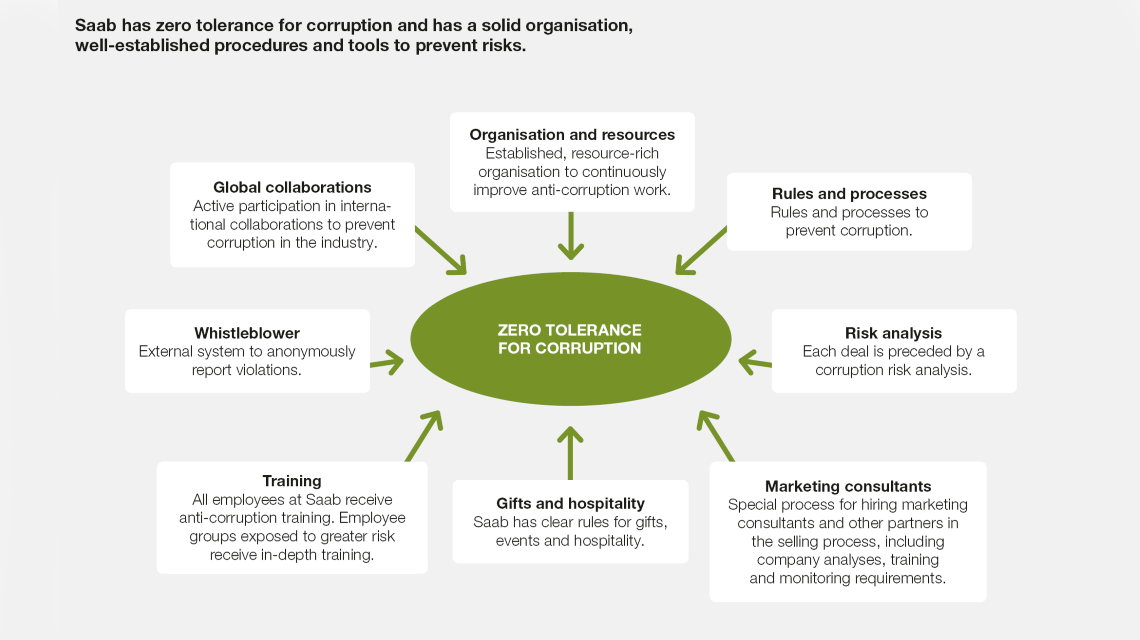
\includegraphics[scale=1.4]{grafik/modell_zero_corruption_1140x640.png}
	\caption{Zero tolerance}\label{fig:zerotolerance}
\end{figure}  
\\
Till exempel gör Saab alltid riskanalyser i samband med affärer för avgöra om det finns risk för korruption. De undersöker risker med vart affären äger rum, vem köparen är, hur upphandlingen går till och hur köparen kom i kontakt med företaget. Om riskerna inte gick att eliminera eller inte var hanterbara drar sig Saab ur affären. Detta är en åtgärd för att förhindra att produkterna hamnar i fel händer. 
\newline
\newline
När utomstående parter är iblandade och flödet av pengar inte är helt under Saabs kontroll finns det alltid risker att produkterna kan hamna i fel händer. För att minimera riskerna ser Saab till att deras etiska värden och riktlinjer strikt följs av utomstående/tillfälligt anställda konsulter och partners. Dessa partners måste genomgå utbildning och skriva under att följa Saabs etiska värden och riktlinjer. I avtalen ingår det att Saab har rätt till att kontrollera om riktlinjerna verkligen följs.   
\newline
\newline
För att förhindra korruption inom företaget utbildar Saab all personal inom ämnet. De har även ett system kallat ''Whistleblower'' för att rapportera suspekta aktiviteter och som garanterar rapporterarens anonymitet.              
\newline
\newline
Utöver vapen levererar Saab bland annat system för väderstationer, minröjning och att detektera kemiska, biologiska, radioaktiva samt kärnvapen. \citep{security}

\subsubsection{Miljöaspekter}
Vårat projekt är inte en skada för miljön eftersom det endast är samling algoritmer för att lösa och visualisera optimeringsproblem.  
\newline
\newline
Om Saab skulle använda vårat projekt i jaktflygplanet JAS 39 Gripen som projektet härstammar ifrån, uppkommer frågor kring hur pass miljövänliga företaget Saab och Gripen är. På deras hemsida \citep{saabimpact} kan man läsa om deras arbete för att minska avtrycket på miljön. De har till exempel satt upp som mål att reducera deras koldioxidutsläpp från försäljningar med tjugo procent till år 2020. I figur~\ref{fig:saabkoldioxid} visas Saabs koldioxidutsläpp och deras mål.   
\leavevmode
\begin{figure}[h]
	\centering
	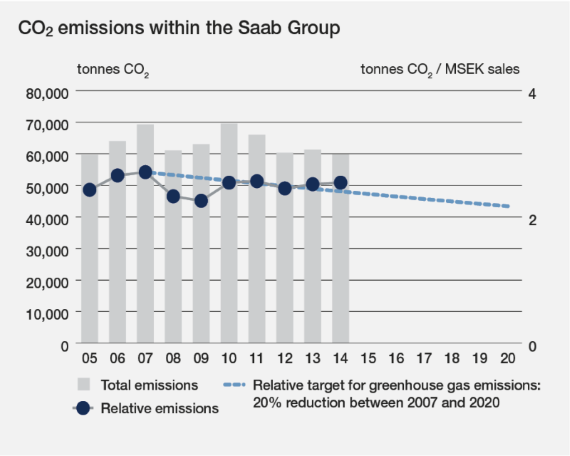
\includegraphics[scale=1.5]{grafik/saabemissions.png}
	\caption{Saabs koldioxidutsläpp}\label{fig:saabkoldioxid}	
\end{figure} 
\\
För att nå målet arbetar Saab med att reducera elförbrukningen på deras fabriker och utsläpp från resor vilka är de största faktorerna för deras koldioxidutsläpp. Genom att fokusera på att ändra de anställdas vanor, ny teknik och strategisk planering av fabrikerna har de lyckats sänka koldioxidutsläppen från fabrikerna med tjugo procent mellan åren 2009 och 2014. För att minska utsläppen från resor nämner Saab bland annat att de uppmuntrar resfria möten och samåkningar.
\newline
\newline 
Deras hantering av miljöfarliga ämnen möter EU's förordning REACH (Registration, Evaluation and Authorisation of Chemicals) som strävar efter att förbättra skyddet av människors hälsa och miljön från risker som kan förorsakas av kemikalier \citep{reach}. 
Saab är även kontributör till projektet Clean Sky som är det mest ambitiösa luftfartsforskningsprogrammet i Europa. Målet med Clean Sky är att utveckla ny teknik för att göra luftfarten mer miljövänlig med mindre bullriga och mer bränsleeffektiva flygplan. \citep{cleansky}     
\newline
\newline
Stridsflygplanet JAS 39 Gripen använder i dagsläget en jetmotor som drivs på fotogen. Fotogen är ett fossilt bränsle som leder till koldioxidutsläpp vid förbränning. Detta gör Gripen till ett system som bidrar till miljöförstöring. 
\newline
\newline
Det verkar som att Saab har ambitioner om att själva bli miljövänligare och att bidra till utvecklingen av miljövänligare teknik. De gör dock fortfarande ett negativt avtryck på miljön eftersom det sker utsläpp av koldioxid och de använder miljöfarliga ämnen i deras produkter. Detta kan dock ses som en direkt följd av att det idag tyvärr inte är lönnsamt att använda eller existerar effektiv miljövänlig el och teknik.  
\newline
\newline
Skulle användadet av vårat projekt göra någon skillnad? Detta går tyvärr inte att svara på då vi saknar uppgifter på hur våran optimeringslösare skulle bidra till miljövänligheten hos stridsflygplanet JAS 39 Gripen.        